% !TeX encoding = UTF-8
% !TeX program = XeLaTeX
% !TeX spellcheck = en_US

\documentclass[english]{../TexTemplate/thesis}
\usepackage{../TexTemplate/mypackage}
\usepackage{ctex}

\title{Week 4 - \LaTeX{} Configuration \& Usage}
\author{Hongzheng Chen}
\date{Dec 6, 2019}
\headercontext{Week 4 - \LaTeX{} Configuration \& Usage}

\begin{document}

\maketitle

Week 4's seminar is partly based on Week00 of \href{https://github.com/pppppass/ToolsSeminar}{ToolsSeminar} held in PKU.
 
\section{Installation and configuration}
For \TeX{} distribution, \href{http://www.tug.org/texlive/}{\TeX{} Live} is an official comprehensive TeX distribution system, which provides system-specific supports.

For Windows and Linux, reading through \href{http://www.tug.org/texlive/acquire-netinstall.html}{installing \TeX{} Live over the Internet} is recommended. A (non-necessary) introduction to \TeX{} Live on Windows is provided \href{http://www.tug.org/texlive/windows.html}{here}. If you are going to install \TeX{} Live on Linux, please read \href{http://www.tug.org/texlive/quickinstall.html}{this page} first, which gives detailed guidance. Installing on your home directory (\verb"/home/someone/texlive/2017" to be exact) instead of default \verb"/usr/local/texlive/2017" is recommended in case of authority issues.

For macOS, please install \href{http://www.tug.org/mactex/}{MacTeX}, which is specially adapted to macOS and includes \TeX{} Live.

Installation information can also be found in \href{https://item.jd.com/11258469.html}{\emph{\LaTeX 入门}}.

Note that there are also alternatives for installation, like \href{http://www.ctex.org/CTeX}{CTeX}, which a suite specialized to Chinese and can be downloaded \href{http://www.ctex.org/CTeXDownload}{here}. However, CTeX is somehow out-of-date now and has no advantages due to the development of XeTeX and LuaTeX.
PdfTex, XeTeX, and LuaTeX are the most widely used \LaTeX{} engines, which have all been integrated into \TeX{} Live.
The differences between them can be found in \href{https://www.overleaf.com/learn/latex/Articles/The_TeX_family_tree:_LaTeX,_pdfTeX,_XeTeX,_LuaTeX_and_ConTeXt}{\emph{The TeX family tree: LaTeX, pdfTeX, XeTeX, LuaTeX and ConTeXt}}.

VS Code has a \LaTeX{} extension called \href{https://marketplace.visualstudio.com/items?itemName=James-Yu.latex-workshop}{LaTeX Workshop}, which is extremely powerful with lots of functions like different engines support, side view of PDF file, and snippet panel. Sublime Text also has \LaTeX{} support by LaTeXTools package.

If you do not want to install \LaTeX{} distributions on your computer, you can use online \LaTeX{} editors like \href{https://www.overleaf.com}{Overleaf} and \href{https://www.sharelatex.com/}{ShareLaTeX}\footnote{ShareLaTeX has been merged with Overleaf and becomes Overleaf v2. Our server installed the open-sourced ShareLaTeX, and you can register from the webpage.}, which are very useful when you write papers or experimental reports with others.
The main drawback is that their servers are mostly abroad, which leads to frequent network breakdown.
Moreover, Overleaf only supports two people collaboration if you use the free version.


\section{Introductions and Tutorials}
The book \href{https://item.jd.com/11258469.html}{\emph{\LaTeX 入门}} is a useful book for anyone using \LaTeX. Not only is the book a complete tutorial, but it also works as an index to frequently used packages. Only chapter 1 is suggested for the first reading, while other chapters, which are filled with details, may be used as a manual.

The Wikibook \href{https://en.wikibooks.org/wiki/LaTeX}{\emph{\LaTeX}} is featured on Wikibooks, providing a brief introduction to \LaTeX. Overleaf's \href{https://www.overleaf.com/learn/latex/Learn_LaTeX_in_30_minutes}{\emph{Learn \LaTeX in 30 Minutes}} also gives basic usage of \LaTeX, and its \href{https://www.overleaf.com/learn/latex/Main_Page}{main page} can be used for manual and guidance. \href{https://liam.page/2014/09/08/latex-introduction/}{一份其实很短的\LaTeX{}入门文档} is a very easy-to-understand tutorial of \LaTeX{} in Chinese.

Note that \TeX{} Live itself includes a documentation system, which can be accessed by the command \verb"texdoc <name>".

The famous \href{https://www.ctan.org/tex-archive/info/lshort/english/}{\emph{The not so Short Introduction to \LaTeX}} is an introduction of moderate length. There is also a \href{ https://www.ctan.org/tex-archive/info/lshort/chinese}{Chinese translation}. It can be directly accessed by \verb"texdoc lshort" and\\ \verb"texdoc lshort-chinese".

By utilizing \verb"texdoc", one may access the document of packages and document classes. For example, executing \verb"texdoc ctex" on a terminal, the documentation of the package \verb"ctex" shows up.

Some other important reference can be accessed by \verb"texdoc". \href{https://www.ctan.org/tex-archive/info/symbols/comprehensive/}{\emph{The Comprehensive \LaTeX{} Symbol List}} can be accessed by \verb"texdoc comprehensive", which lists many symbols. \href{https://www.ctan.org/pkg/maths-symbols}{\emph{Summary of Mathmatical Symbols available in \LaTeX}} can be accessed by \verb"texdoc symbols", which is a compact summary of \LaTeX{} symbols. Further information of \TeX{} Live can be found by \verb"texdoc texlive".

For websites, \href{https://tex.stackexchange.com/}{TeX StackExchange} is a community for \TeX{} and \LaTeX{} users, which is very helpful for hard \TeX{} and \LaTeX{} questions and practical tricks.
\href{https://zhuanlan.zhihu.com/LaTeX}{Zhihu} also has lots of topics on \LaTeX{}, and the author of \href{https://item.jd.com/11258469.html}{\emph{\LaTeX 入门}} is active on it.


\section{Packages and Templates}
TeXLive has pre-installed most of the packages you need to use, so you only need to include them by \verb'\usepackage{...}' in the preamble part.
For templates, you can find a lot on \href{LaTeX studio}. Or you can download the \href{https://github.com/chhzh123/mylatextmpl}{\LaTeX{} templates} designed by me for daily note, slide, and class reports usage.
You can also find these templates in \verb'TeXTemplate' of the seminar folder.

Once you download others' templates (\verb'.cls' or \verb'.sty'), you can put them in the current folder with your document and directly include them, or you can put them in the \verb'texmf' folder to make them work globally (refer to \href{https://marquistj13.github.io/MyBlog/2017/04/install-latex-cls/}{this page}).

Beamer is the document class for making slides, you can refer to Overleaf's \href{https://www.overleaf.com/learn/latex/Beamer_Presentations:_A_Tutorial_for_Beginners_(Part_1)\%E2\%80\%94Getting_Started}{tutorial} for more details.
Default themes can be found in \href{http://deic.uab.es/~iblanes/beamer_gallery/}{Beamer theme gallery} and \href{https://hartwork.org/beamer-theme-matrix/}{Beamer theme matrix}.
For beamer templates, you can find \href{https://www.latexstudio.net/archives/category/tex-slides/beamer-theme-template}{here}.

The commonly used packages are listed in the slide.
For most of the packages, you can find their manuals and documentation on \href{https://ctan.org/}{CTan}.
If you don't know how to format some paragraphs with specific styles, use Google to search for that.


\section{Other Useful Things}
If you carefully configure \LaTeX{} environment and define macros, you can definitely use \LaTeX{} to take notes at school. As an example, you can see the \href{https://github.com/chhzh123/Notes-of-Math}{math notes} taken by me, which are all in \LaTeX{} format.
About how to take \LaTeX{} notes quickly, you can see this \href{https://castel.dev/post/lecture-notes-1/}{blog}, the author of which use \LaTeX{} and Vim to take more than 1700 pages of notes on his math courses.

Apart from the snippet panel provided by VS Code's extension, another quick page searching math functions can be found \href{https://katex.org/docs/supported.html}{here}. Once you use them frequently, you will easily remember their abbreviations and write \LaTeX{} documents much faster.

Some Optical Character Recognition (OCR) techniques are used to free programmers from tedious \LaTeX{} formula typing, including \href{https://mathpix.com/}{Mathpix} and \href{http://detexify.kirelabs.org/classify.html}{Detexify}.
Also, \href{https://www.wolfram.com/mathematica}{Mathematica} supports direct translation from Wolfram formulas to \LaTeX{} commands.

\href{https://www.tablesgenerator.com/}{Tables Generator} and Excel2LaTeX (\href{http://excel2latex.com/}{online}, \href{https://ctan.org/pkg/excel2latex?lang=en}{macro}) are used for generating tables from Excels to \LaTeX{} quickly. But these tools both cannot handle complex tables with lots of merged units.

Markdown inherently supports \LaTeX{} if the website has included the script of \href{https://katex.org/}{KaTeX} or \href{https://www.mathjax.org/}{MathJax}. You can write \LaTeX{} symbols in Markdown as if in \LaTeX{} editors. Inline formulas are enclosed by \verb'$...$', while \verb'$$...$$' is used for displayed ones.

Last but not least, when you are writing \LaTeX{} in Chinese or English, there are lots of specifications you need to pay attention to, which can be referred by \href{https://web.stanford.edu/class/ee364b/latex_templates/template_notes.pdf}{\emph{\LaTeX{} Style Guide for EE 364B}}, \href{https://www.ams.org/publications/authors/AMS-StyleGuide-online.pdf}{\emph{AMS Style Guide}}, and \href{https://zhuanlan.zhihu.com/p/29587837}{this article} in Chinese.


\newpage
\section{Assignment}
In this week's assignment, you need to use \LaTeX{} to generate two documents, one for Chinese notes, and another for English academic paper.
Once you finished, the source \verb'tex' files and the generated \verb'pdf' files should all be pushed to Github.

\subsection{Chinese Notes}
You need to start from scratch and generate the note shown below, which consists of two questions and answers extracted from your math books.
The pdf file is attached in \verb'Assignments/LaTeX/exe_ch.pdf'.
\begin{figure}[H]
\centering
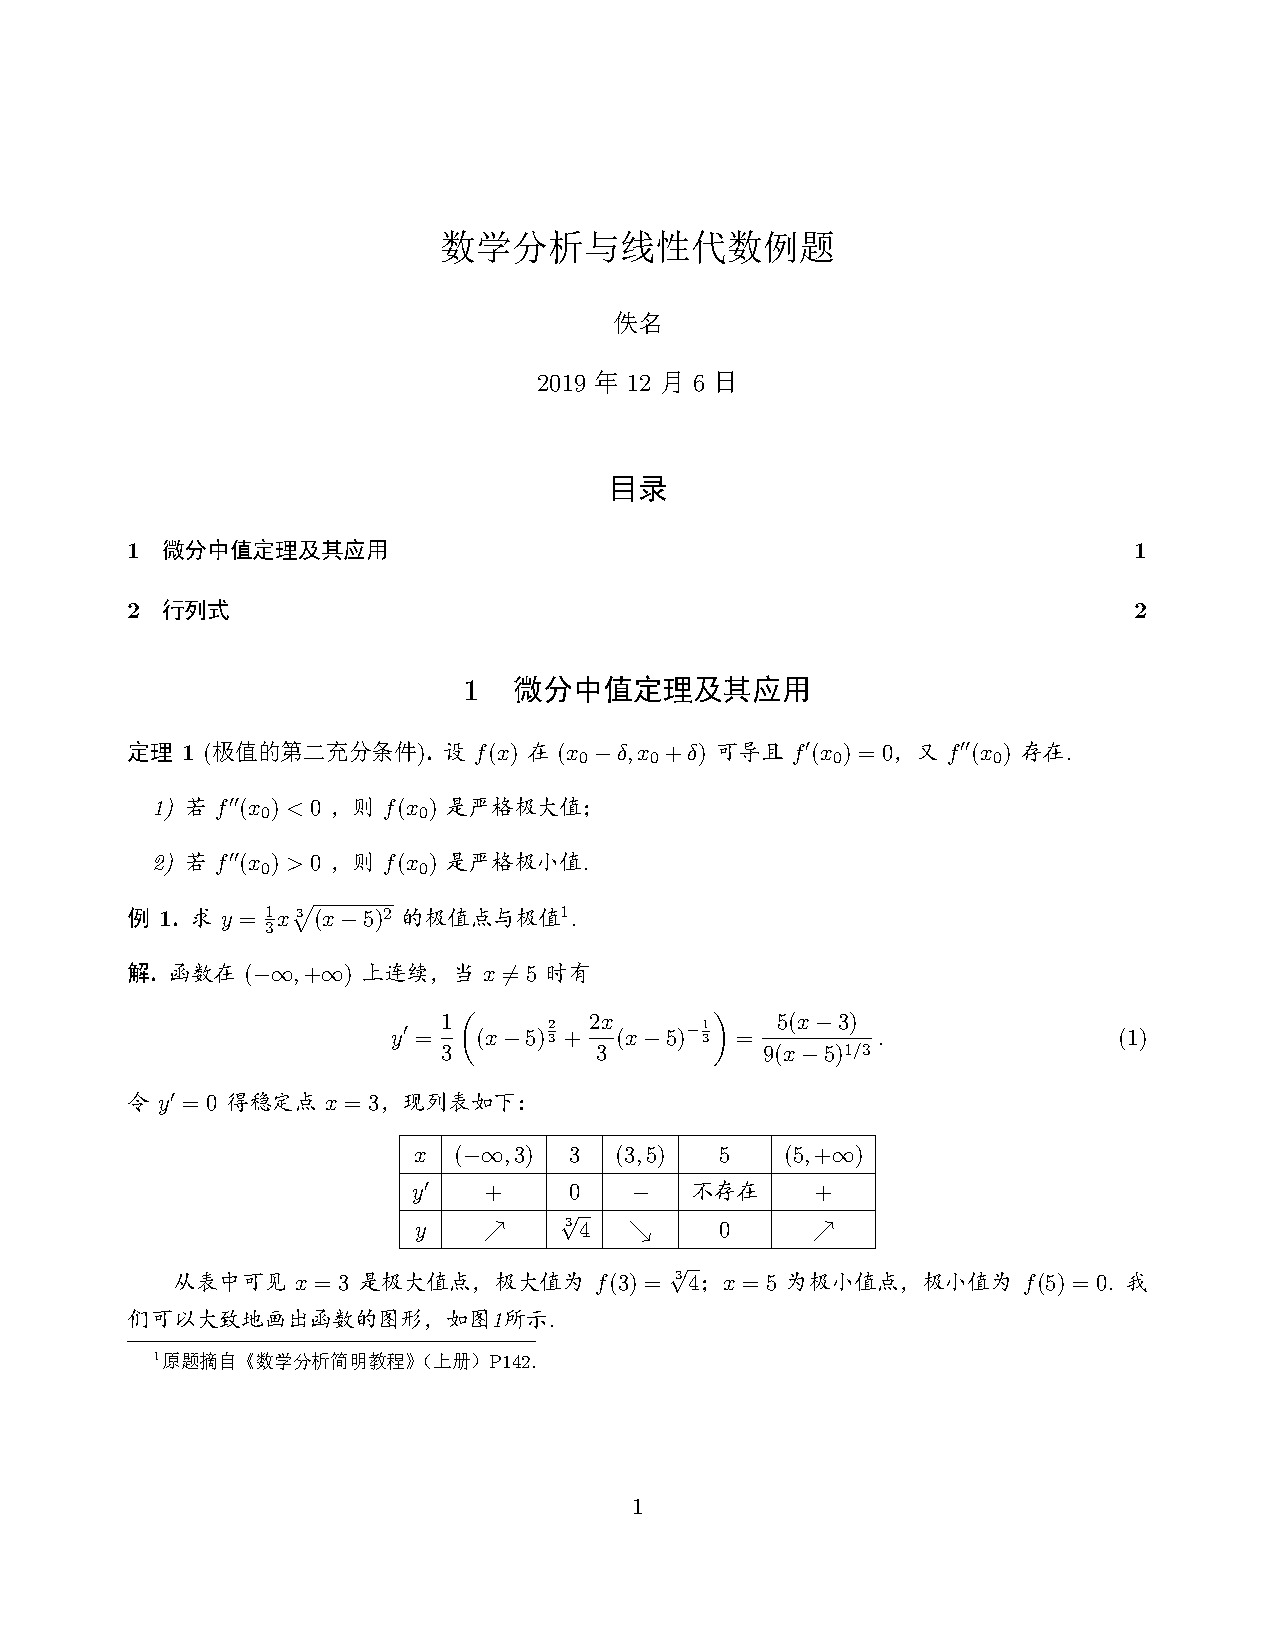
\includegraphics[width=0.7\linewidth]{../Assignments/LaTeX/exe_ch.pdf}
\end{figure}

You should make your generated contents \emph{as similar as} those in \verb'exe_ch.pdf'.
Some hints:
\begin{enumerate}
	\item Use \verb'\documentclass[UTF8,11pt]{ctexart}'.
	\item Include the following packages:
	\begin{itemize}
		\item \verb'amsthm' for theorem environment.
		\item \verb'amsfonts' for bold math symbols.
		\item \verb'amsmath' for matrix environment.
		\item \verb'graphicx' for figure environment.
		\item \verb'geometry' for page size, and put \verb'\geometry{scale=0.8}' in preamble.
	\end{itemize}
	\item Insert whitespaces between Chinese and formulas, but no spaces between Chinese and punctuation marks are needed.
	\item Even in Chinese article, you should use \verb'.' as period.
	\item Use sth. like 图\verb'\ref{fig:1}' to cross reference (including figures, equations, and tables). Avoid directly writing 图 1.
	\item Figures commonly use \verb'[htbp]' to align, meaning try putting \underline{h}ere first, then \underline{t}op, \underline{b}ottom, and next \underline{p}age. For more about alignment of floating environments, you can refer to \href{http://web.mit.edu/molly/Public/mini/figtab.pdf}{MIT FigTab} or \href{https://tex.stackexchange.com/questions/2275/keeping-tables-figures-close-to-where-they-are-mentioned}{TeX Stackexchange}.
	\item If the equations have numbering at the right, use \verb'equation' environment.
	Otherwise, you can directly use \verb'\[...\]' for display.
	\item Commonly, vectors use bold notation like $\mathbf{x}$ (\verb'\mathbf{...}') and sets use blackboard bold typeface like $\mathbb{R}$ (\verb'\mathbb{...}'). Math operations are in straight font like $\log$ (\verb'$\log$') not $log$ (\verb'$log$') in Italic font.
	\item Using \verb'\left(...\right)' can make the parenthesis larger.
	\item The figure needed inserting is provided in \verb'Assignments/LaTeX/fig/function.pdf'.
	\item Be careful about whether the symbols are in displayed mode.
	\item If you do not know how to type some specific symbols, please find \href{https://katex.org/docs/supported.html}{here}.
\end{enumerate}

\subsection{English Academic Paper}
You need to use the ACM conference template to generate a short academic paper shown below.
The pdf file is attached in \verb'Assignments/LaTeX/exe_en.pdf'.
\begin{figure}[!t]
\centering
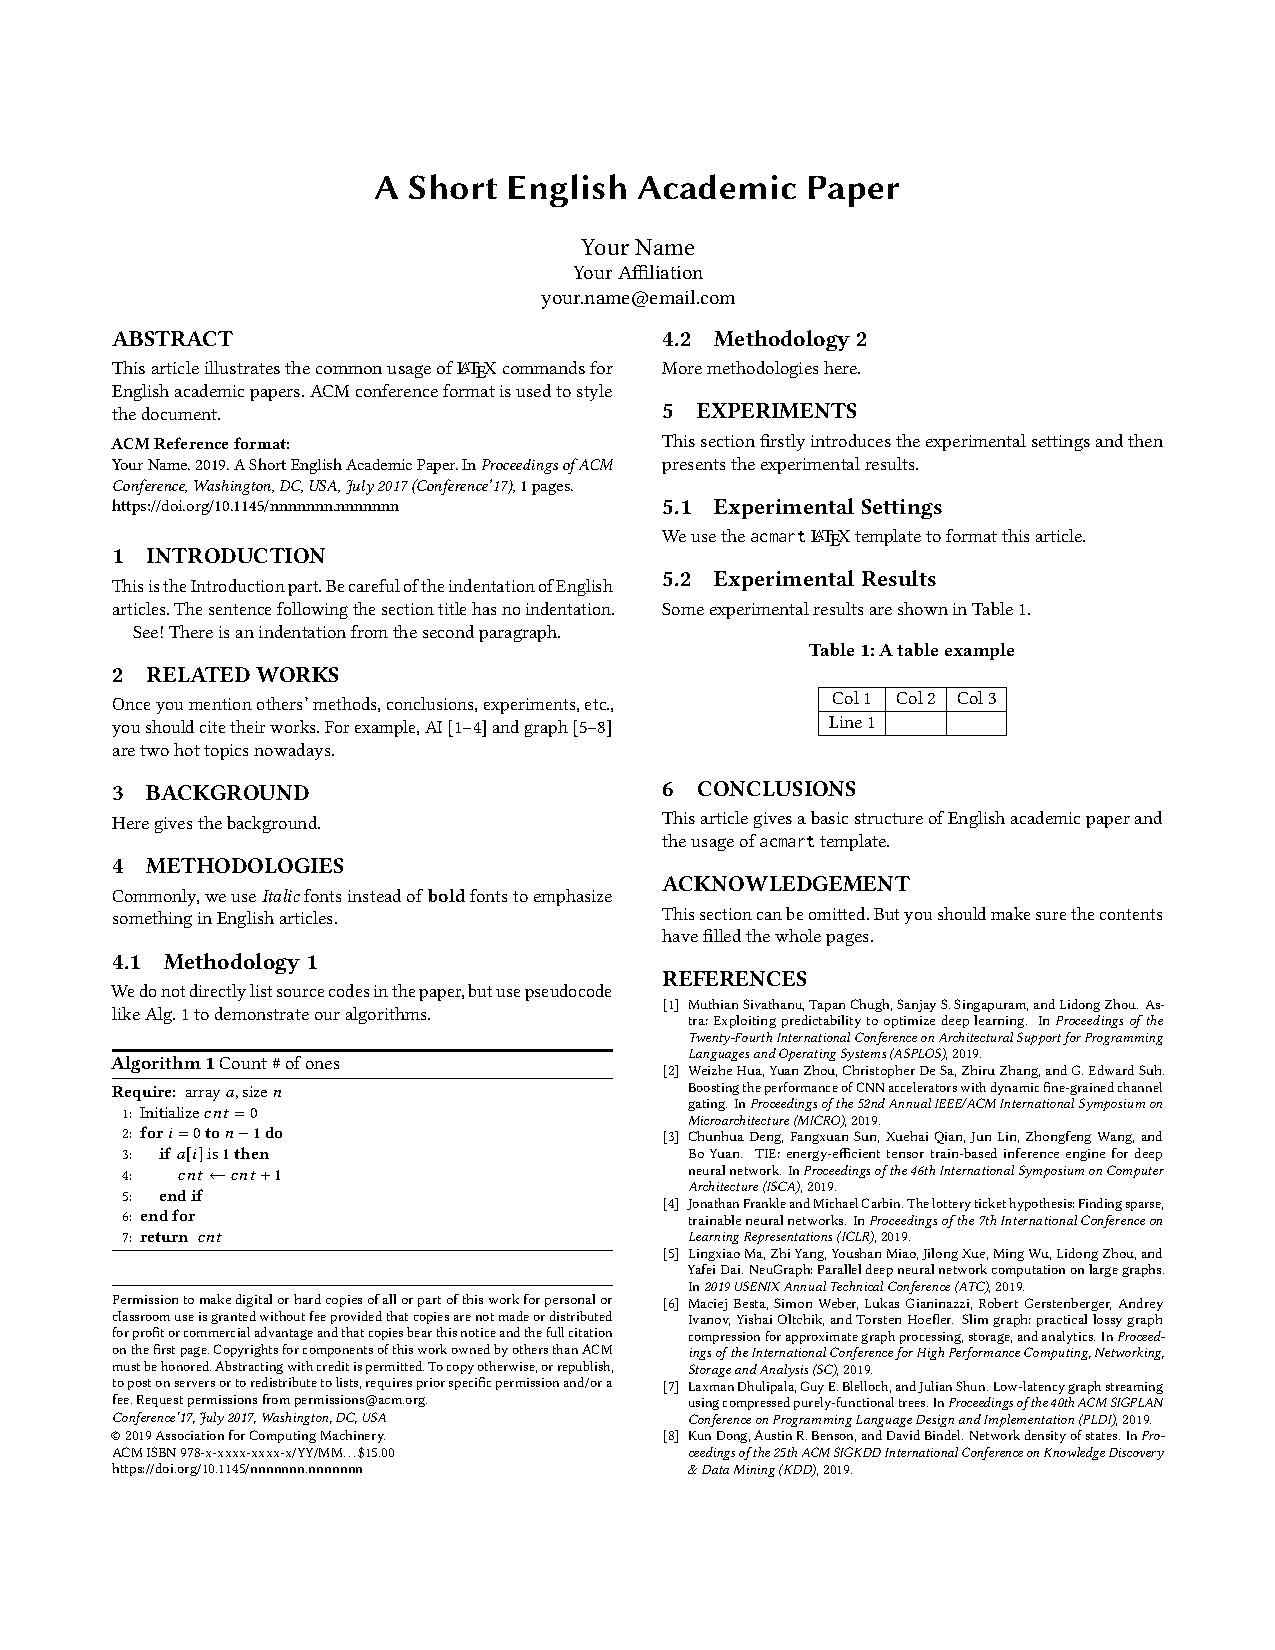
\includegraphics[width=0.7\linewidth]{../Assignments/LaTeX/exe_en.pdf}
\end{figure}

Some hints:
\begin{enumerate}
	\item The template file \verb'acmart.cls' is provided, or you can directly use \verb'\documentclass[sigconf]{acmart}' if you have installed the TeXLive distribution.
	\item \verb'sample-sigconf.tex' is an official sample provided by ACM.
	You can follow this sample to generate the corresponding pdf.
	\item \verb'algorithm' and \verb'algorithmic' packages are used for generating pseudocode. Their usage can be found in \href{https://www.overleaf.com/learn/latex/algorithms}{Overleaf} or \href{https://en.wikibooks.org/wiki/LaTeX/Algorithms}{Wikibooks}.
	\item Use your \verb'bib' file in Week 2 to generate cites and references, and the \verb'bibliographystyle' should be set to \verb'unsrt' making sure the cites are in order.
	\item Your \verb'bib' file should at least include \verb'title', \verb'booktitle', \verb'author', and \verb'year' keys for each item.
	And all these items should use \verb'@inproceedings' format. Otherwise, your generated file will be different from the provided pdf.
	\item All the citations and reference of tables, algorithms, figures, etc., should use cross reference, i.e. \verb'\cite{...}' and \verb'\ref{...}'.
\end{enumerate}

\end{document}